\documentclass{beamer}
\usepackage{tikz}
\usetikzlibrary{external}
\tikzexternalize
\usepackage{xcolor}

%Paper Node
\makeatletter
\pgfdeclareshape{document}{
\inheritsavedanchors[from=rectangle] % this is nearly a rectangle
\inheritanchorborder[from=rectangle]
\inheritanchor[from=rectangle]{center}
\inheritanchor[from=rectangle]{north}
\inheritanchor[from=rectangle]{south}
\inheritanchor[from=rectangle]{west}
\inheritanchor[from=rectangle]{east}
% ... and possibly more
\backgroundpath{% this is new
% store lower right in xa/ya and upper right in xb/yb
\southwest \pgf@xa=\pgf@x \pgf@ya=\pgf@y
\northeast \pgf@xb=\pgf@x \pgf@yb=\pgf@y
% compute corner of ‘‘flipped page’’
\pgf@xc=\pgf@xb \advance\pgf@xc by-7pt % this should be a parameter
\pgf@yc=\pgf@yb \advance\pgf@yc by-7pt
% construct main path
\pgfpathmoveto{\pgfpoint{\pgf@xa}{\pgf@ya}}
\pgfpathlineto{\pgfpoint{\pgf@xa}{\pgf@yb}}
\pgfpathlineto{\pgfpoint{\pgf@xc}{\pgf@yb}}
\pgfpathlineto{\pgfpoint{\pgf@xb}{\pgf@yc}}
\pgfpathlineto{\pgfpoint{\pgf@xb}{\pgf@ya}}
\pgfpathclose
% add little corner
\pgfpathmoveto{\pgfpoint{\pgf@xc}{\pgf@yb}}
\pgfpathlineto{\pgfpoint{\pgf@xc}{\pgf@yc}}
\pgfpathlineto{\pgfpoint{\pgf@xb}{\pgf@yc}}
\pgfpathlineto{\pgfpoint{\pgf@xc}{\pgf@yc}}
}
}
\makeatother

\makeatletter
\newcommand*{\overlaynumber}{\number\beamer@slideinframe}
\tikzset{
  beamer externalizing/.style={%
    execute at end picture={%
      \tikzifexternalizing{%
        \ifbeamer@anotherslide
        \pgfexternalstorecommand{\string\global\string\beamer@anotherslidetrue}%
        \fi
      }{}%
    }%
  },
  external/optimize=false
}
\let\orig@tikzsetnextfilename=\tikzsetnextfilename
\renewcommand\tikzsetnextfilename[1]{\orig@tikzsetnextfilename{#1-\overlaynumber}}
\makeatother

\begin{document}
\begin{frame}{Image}
\begin{figure}[htpb]
    \centering
    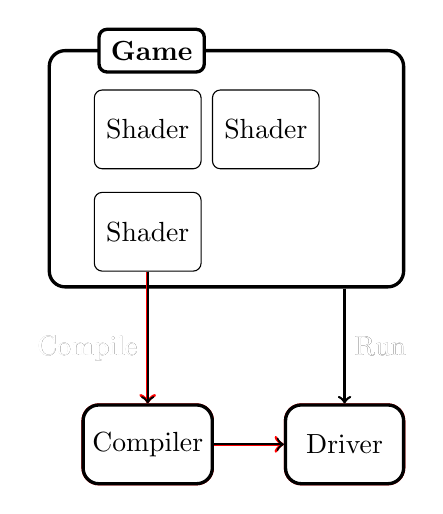
\begin{tikzpicture}
        % Surrounding
        % draw=white
        %\node [rounded corners=2mm, thick, draw=black, fill=white, opacity=0.4, minimum width=55mm, minimum height=40mm, align=center] at (0,0) (sur) {};

        % Game
        \node [rounded corners=2mm, very thick, fill=white, draw=black, minimum width=45mm, minimum height=30mm, align=center] at (0, 0) (game) {};
        \node [rounded corners=1mm, very thick, fill=white, draw=black, inner sep=1.5mm, xshift=-9.5mm, yshift=15mm] at (game) {\textbf{Game}};
        \node [rounded corners=1mm, draw=black, inner sep=1.5mm, xshift=-10mm, yshift=5mm, minimum height=10mm] at (game) {Shader};
        \node [rounded corners=1mm, draw=black, inner sep=1.5mm, xshift=5mm, yshift=5mm, minimum height=10mm] at (game) {Shader};
        \node [rounded corners=1mm, draw=black, inner sep=1.5mm, xshift=-10mm, yshift=-8mm, minimum height=10mm] at (game) (shader) {Shader};

        % Compiler
        \alt<3>{
            \node [rounded corners=2mm, very thick, fill=white!80!red, draw=red, minimum width=15mm, minimum height=10mm, align=center] at (-10mm, -35mm) (compiler) {Compiler};
        }{
            \node [rounded corners=2mm, very thick, fill=white, draw=black, minimum width=15mm, minimum height=10mm, align=center] at (-10mm, -35mm) (compiler) {Compiler};
        }

        \alt<5>{
            \node [rounded corners=2mm, very thick, fill=white!80!red, draw=red, minimum width=15mm, minimum height=10mm, align=center] at (15mm, -35mm) (driver) {Driver};
        }{
            \node [rounded corners=2mm, very thick, fill=white, draw=black, minimum width=15mm, minimum height=10mm, align=center] at (15mm, -35mm) (driver) {Driver};
        }

        \alt<1>{
            \draw[->, thick] (shader) -- node[left, yshift=-1.4mm] {Compile} (compiler);
        }{
            \alt<2>{
                \draw[->, very thick, text=white, draw=red] (shader) -- node[left, yshift=-1.4mm] {Compile} (compiler);
            }{
                \draw[->, thick, text=white] (shader) -- node[left, yshift=-1.4mm] {Compile} (compiler);
            }
        }
        \alt<4>{
            \draw[->, very thick, draw=red] (compiler) -- (driver);
        }{
            \draw[->, thick] (compiler) -- (driver);
        }
        \alt<1>{
            \draw[->, thick] (game.south-|driver) -- node[right] {Run} (driver);
        }{
            \draw[->, thick, text=white] (game.south-|driver) -- node[right] {Run} (driver);
        }
    \end{tikzpicture}
\end{figure}
\only<5>{}
\end{frame}
\end{document}
